\documentclass[1p]{elsarticle_modified}
%\bibliographystyle{elsarticle-num}

%\usepackage[colorlinks]{hyperref}
%\usepackage{abbrmath_seonhwa} %\Abb, \Ascr, \Acal ,\Abf, \Afrak
\usepackage{amsfonts}
\usepackage{amssymb}
\usepackage{amsmath}
\usepackage{amsthm}
\usepackage{scalefnt}
\usepackage{amsbsy}
\usepackage{kotex}
\usepackage{caption}
\usepackage{subfig}
\usepackage{color}
\usepackage{graphicx}
\usepackage{xcolor} %% white, black, red, green, blue, cyan, magenta, yellow
\usepackage{float}
\usepackage{setspace}
\usepackage{hyperref}

\usepackage{tikz}
\usetikzlibrary{arrows}

\usepackage{multirow}
\usepackage{array} % fixed length table
\usepackage{hhline}

%%%%%%%%%%%%%%%%%%%%%
\makeatletter
\renewcommand*\env@matrix[1][\arraystretch]{%
	\edef\arraystretch{#1}%
	\hskip -\arraycolsep
	\let\@ifnextchar\new@ifnextchar
	\array{*\c@MaxMatrixCols c}}
\makeatother %https://tex.stackexchange.com/questions/14071/how-can-i-increase-the-line-spacing-in-a-matrix
%%%%%%%%%%%%%%%

\usepackage[normalem]{ulem}

\newcommand{\msout}[1]{\ifmmode\text{\sout{\ensuremath{#1}}}\else\sout{#1}\fi}
%SOURCE: \msout is \stkout macro in https://tex.stackexchange.com/questions/20609/strikeout-in-math-mode

\newcommand{\cancel}[1]{
	\ifmmode
	{\color{red}\msout{#1}}
	\else
	{\color{red}\sout{#1}}
	\fi
}

\newcommand{\add}[1]{
	{\color{blue}\uwave{#1}}
}

\newcommand{\replace}[2]{
	\ifmmode
	{\color{red}\msout{#1}}{\color{blue}\uwave{#2}}
	\else
	{\color{red}\sout{#1}}{\color{blue}\uwave{#2}}
	\fi
}

\newcommand{\Sol}{\mathcal{S}} %segment
\newcommand{\D}{D} %diagram
\newcommand{\A}{\mathcal{A}} %arc


%%%%%%%%%%%%%%%%%%%%%%%%%%%%%5 test

\def\sl{\operatorname{\textup{SL}}(2,\Cbb)}
\def\psl{\operatorname{\textup{PSL}}(2,\Cbb)}
\def\quan{\mkern 1mu \triangleright \mkern 1mu}

\theoremstyle{definition}
\newtheorem{thm}{Theorem}[section]
\newtheorem{prop}[thm]{Proposition}
\newtheorem{lem}[thm]{Lemma}
\newtheorem{ques}[thm]{Question}
\newtheorem{cor}[thm]{Corollary}
\newtheorem{defn}[thm]{Definition}
\newtheorem{exam}[thm]{Example}
\newtheorem{rmk}[thm]{Remark}
\newtheorem{alg}[thm]{Algorithm}

\newcommand{\I}{\sqrt{-1}}
\begin{document}

%\begin{frontmatter}
%
%\title{Boundary parabolic representations of knots up to 8 crossings}
%
%%% Group authors per affiliation:
%\author{Yunhi Cho} 
%\address{Department of Mathematics, University of Seoul, Seoul, Korea}
%\ead{yhcho@uos.ac.kr}
%
%
%\author{Seonhwa Kim} %\fnref{s_kim}}
%\address{Center for Geometry and Physics, Institute for Basic Science, Pohang, 37673, Korea}
%\ead{ryeona17@ibs.re.kr}
%
%\author{Hyuk Kim}
%\address{Department of Mathematical Sciences, Seoul National University, Seoul 08826, Korea}
%\ead{hyukkim@snu.ac.kr}
%
%\author{Seokbeom Yoon}
%\address{Department of Mathematical Sciences, Seoul National University, Seoul, 08826,  Korea}
%\ead{sbyoon15@snu.ac.kr}
%
%\begin{abstract}
%We find all boundary parabolic representation of knots up to 8 crossings.
%
%\end{abstract}
%\begin{keyword}
%    \MSC[2010] 57M25 
%\end{keyword}
%
%\end{frontmatter}

%\linenumbers
%\tableofcontents
%
\newcommand\colored[1]{\textcolor{white}{\rule[-0.35ex]{0.8em}{1.4ex}}\kern-0.8em\color{red} #1}%
%\newcommand\colored[1]{\textcolor{white}{ #1}\kern-2.17ex	\textcolor{white}{ #1}\kern-1.81ex	\textcolor{white}{ #1}\kern-2.15ex\color{red}#1	}

{\Large $\underline{12n_{0757}~(K12n_{0757})}$}

\setlength{\tabcolsep}{10pt}
\renewcommand{\arraystretch}{1.6}
\vspace{1cm}\begin{tabular}{m{100pt}>{\centering\arraybackslash}m{274pt}}
\multirow{5}{120pt}{
	\centering
	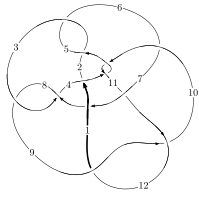
\includegraphics[width=112pt]{../../../GIT/diagram.site/Diagrams/png/2846_12n_0757.png}\\
\ \ \ A knot diagram\footnotemark}&
\allowdisplaybreaks
\textbf{Linearized knot diagam} \\
\cline{2-2}
 &
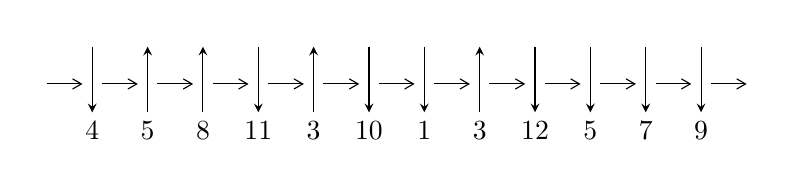
\begin{tikzpicture}[x=20pt, y=17pt]
	% nodes
	\node (C0) at (0, 0) {};
	\node (C1) at (1, 0) {};
	\node (C1U) at (1, +1) {};
	\node (C1D) at (1, -1) {4};

	\node (C2) at (2, 0) {};
	\node (C2U) at (2, +1) {};
	\node (C2D) at (2, -1) {5};

	\node (C3) at (3, 0) {};
	\node (C3U) at (3, +1) {};
	\node (C3D) at (3, -1) {8};

	\node (C4) at (4, 0) {};
	\node (C4U) at (4, +1) {};
	\node (C4D) at (4, -1) {11};

	\node (C5) at (5, 0) {};
	\node (C5U) at (5, +1) {};
	\node (C5D) at (5, -1) {3};

	\node (C6) at (6, 0) {};
	\node (C6U) at (6, +1) {};
	\node (C6D) at (6, -1) {10};

	\node (C7) at (7, 0) {};
	\node (C7U) at (7, +1) {};
	\node (C7D) at (7, -1) {1};

	\node (C8) at (8, 0) {};
	\node (C8U) at (8, +1) {};
	\node (C8D) at (8, -1) {3};

	\node (C9) at (9, 0) {};
	\node (C9U) at (9, +1) {};
	\node (C9D) at (9, -1) {12};

	\node (C10) at (10, 0) {};
	\node (C10U) at (10, +1) {};
	\node (C10D) at (10, -1) {5};

	\node (C11) at (11, 0) {};
	\node (C11U) at (11, +1) {};
	\node (C11D) at (11, -1) {7};

	\node (C12) at (12, 0) {};
	\node (C12U) at (12, +1) {};
	\node (C12D) at (12, -1) {9};
	\node (C13) at (13, 0) {};

	% arrows
	\draw[->,>={angle 60}]
	(C0) edge (C1) (C1) edge (C2) (C2) edge (C3) (C3) edge (C4) (C4) edge (C5) (C5) edge (C6) (C6) edge (C7) (C7) edge (C8) (C8) edge (C9) (C9) edge (C10) (C10) edge (C11) (C11) edge (C12) (C12) edge (C13) ;	\draw[->,>=stealth]
	(C1U) edge (C1D) (C2D) edge (C2U) (C3D) edge (C3U) (C4U) edge (C4D) (C5D) edge (C5U) (C6U) edge (C6D) (C7U) edge (C7D) (C8D) edge (C8U) (C9U) edge (C9D) (C10U) edge (C10D) (C11U) edge (C11D) (C12U) edge (C12D) ;
	\end{tikzpicture} \\
\hhline{~~} \\& 
\textbf{Solving Sequence} \\ \cline{2-2} 
 &
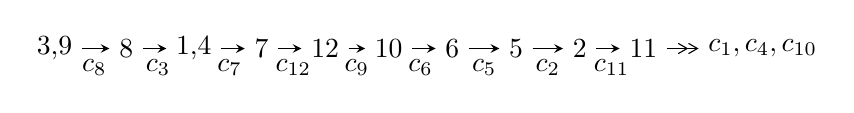
\begin{tikzpicture}[x=23pt, y=7pt]
	% node
	\node (A0) at (-1/8, 0) {3,9};
	\node (A1) at (1, 0) {8};
	\node (A2) at (33/16, 0) {1,4};
	\node (A3) at (25/8, 0) {7};
	\node (A4) at (33/8, 0) {12};
	\node (A5) at (41/8, 0) {10};
	\node (A6) at (49/8, 0) {6};
	\node (A7) at (57/8, 0) {5};
	\node (A8) at (65/8, 0) {2};
	\node (A9) at (73/8, 0) {11};
	\node (C1) at (1/2, -1) {$c_{8}$};
	\node (C2) at (3/2, -1) {$c_{3}$};
	\node (C3) at (21/8, -1) {$c_{7}$};
	\node (C4) at (29/8, -1) {$c_{12}$};
	\node (C5) at (37/8, -1) {$c_{9}$};
	\node (C6) at (45/8, -1) {$c_{6}$};
	\node (C7) at (53/8, -1) {$c_{5}$};
	\node (C8) at (61/8, -1) {$c_{2}$};
	\node (C9) at (69/8, -1) {$c_{11}$};
	\node (A10) at (11, 0) {$c_{1},c_{4},c_{10}$};

	% edge
	\draw[->,>=stealth]	
	(A0) edge (A1) (A1) edge (A2) (A2) edge (A3) (A3) edge (A4) (A4) edge (A5) (A5) edge (A6) (A6) edge (A7) (A7) edge (A8) (A8) edge (A9) ;
	\draw[->>,>={angle 60}]	
	(A9) edge (A10);
\end{tikzpicture} \\ 

\end{tabular} \\

\footnotetext{
The image of knot diagram is generated by the software ``\textbf{Draw programme}" developed by Andrew Bartholomew(\url{http://www.layer8.co.uk/maths/draw/index.htm\#Running-draw}), where we modified some parts for our purpose(\url{https://github.com/CATsTAILs/LinksPainter}).
}\phantom \\ \newline 
\centering \textbf{Ideals for irreducible components\footnotemark of $X_{\text{par}}$} 
 
\begin{align*}
I^u_{1}&=\langle 
-1.59036\times10^{313} u^{84}+4.77989\times10^{312} u^{83}+\cdots+6.91107\times10^{314} b+1.33907\times10^{316},\\
\phantom{I^u_{1}}&\phantom{= \langle  }-9.31472\times10^{316} u^{84}+5.83485\times10^{316} u^{83}+\cdots+8.06522\times10^{317} a+1.67212\times10^{320},\\
\phantom{I^u_{1}}&\phantom{= \langle  }u^{85}+27 u^{83}+\cdots+4868 u+1167\rangle \\
I^u_{2}&=\langle 
-14825031610 u^{27}+18537500123 u^{26}+\cdots+6921637191 b+5273642732,\\
\phantom{I^u_{2}}&\phantom{= \langle  }305534977593367 u^{27}-790948509790679 u^{26}+\cdots+30157573241187 a-1297710378699701,\\
\phantom{I^u_{2}}&\phantom{= \langle  }u^{28}- u^{27}+\cdots- u+1\rangle \\
I^u_{3}&=\langle 
b- u,\;a+u-1,\;u^2- u+1\rangle \\
I^u_{4}&=\langle 
b- u,\;a+u,\;u^2- u+1\rangle \\
\\
\end{align*}
\raggedright * 4 irreducible components of $\dim_{\mathbb{C}}=0$, with total 117 representations.\\
\footnotetext{All coefficients of polynomials are rational numbers. But the coefficients are sometimes approximated in decimal forms when there is not enough margin.}
\newpage
\renewcommand{\arraystretch}{1}
\centering \section*{I. $I^u_{1}= \langle -1.59\times10^{313} u^{84}+4.78\times10^{312} u^{83}+\cdots+6.91\times10^{314} b+1.34\times10^{316},\;-9.31\times10^{316} u^{84}+5.83\times10^{316} u^{83}+\cdots+8.07\times10^{317} a+1.67\times10^{320},\;u^{85}+27 u^{83}+\cdots+4868 u+1167 \rangle$}
\flushleft \textbf{(i) Arc colorings}\\
\begin{tabular}{m{7pt} m{180pt} m{7pt} m{180pt} }
\flushright $a_{3}=$&$\begin{pmatrix}0\\u\end{pmatrix}$ \\
\flushright $a_{9}=$&$\begin{pmatrix}1\\0\end{pmatrix}$ \\
\flushright $a_{8}=$&$\begin{pmatrix}1\\u^2\end{pmatrix}$ \\
\flushright $a_{1}=$&$\begin{pmatrix}0.115492 u^{84}-0.0723458 u^{83}+\cdots-355.666 u-207.324\\0.0230118 u^{84}-0.00691628 u^{83}+\cdots-20.4097 u-19.3757\end{pmatrix}$ \\
\flushright $a_{4}=$&$\begin{pmatrix}u\\u^3+u\end{pmatrix}$ \\
\flushright $a_{7}=$&$\begin{pmatrix}-0.110696 u^{84}+0.130681 u^{83}+\cdots+956.188 u+362.084\\0.0473216 u^{84}+0.0461518 u^{83}+\cdots+828.691 u+175.587\end{pmatrix}$ \\
\flushright $a_{12}=$&$\begin{pmatrix}0.138504 u^{84}-0.0792621 u^{83}+\cdots-376.076 u-226.700\\0.0230118 u^{84}-0.00691628 u^{83}+\cdots-20.4097 u-19.3757\end{pmatrix}$ \\
\flushright $a_{10}=$&$\begin{pmatrix}-0.0884816 u^{84}-0.0814471 u^{83}+\cdots-1489.39 u-309.371\\-0.0199738 u^{84}-0.0308531 u^{83}+\cdots-502.451 u-116.544\end{pmatrix}$ \\
\flushright $a_{6}=$&$\begin{pmatrix}0.0801281 u^{84}+0.0399526 u^{83}+\cdots+844.648 u+163.284\\0.0667657 u^{84}-0.00303016 u^{83}+\cdots+340.400 u+24.5255\end{pmatrix}$ \\
\flushright $a_{5}=$&$\begin{pmatrix}0.0801281 u^{84}+0.0399526 u^{83}+\cdots+844.648 u+163.284\\0.0299497 u^{84}-0.0114804 u^{83}+\cdots+52.4010 u-22.0992\end{pmatrix}$ \\
\flushright $a_{2}=$&$\begin{pmatrix}0.102164 u^{84}-0.0583120 u^{83}+\cdots-240.005 u-161.556\\0.0117585 u^{84}+0.00232467 u^{83}+\cdots+42.4888 u+10.0149\end{pmatrix}$ \\
\flushright $a_{11}=$&$\begin{pmatrix}-0.00514215 u^{84}+0.0946688 u^{83}+\cdots+1138.04 u+304.529\\0.0345003 u^{84}+0.0325184 u^{83}+\cdots+586.871 u+114.297\end{pmatrix}$\\&\end{tabular}
\flushleft \textbf{(ii) Obstruction class $= -1$}\\~\\
\flushleft \textbf{(iii) Cusp Shapes $= -0.274096 u^{84}-0.0366470 u^{83}+\cdots-1775.76 u-145.097$}\\~\\
\newpage\renewcommand{\arraystretch}{1}
\flushleft \textbf{(iv) u-Polynomials at the component}\newline \\
\begin{tabular}{m{50pt}|m{274pt}}
Crossings & \hspace{64pt}u-Polynomials at each crossing \\
\hline $$\begin{aligned}c_{1}\end{aligned}$$&$\begin{aligned}
&u^{85}-5 u^{84}+\cdots-783263 u-43963
\end{aligned}$\\
\hline $$\begin{aligned}c_{2},c_{5}\end{aligned}$$&$\begin{aligned}
&u^{85}+4 u^{84}+\cdots+6399682 u+378351
\end{aligned}$\\
\hline $$\begin{aligned}c_{3},c_{8}\end{aligned}$$&$\begin{aligned}
&u^{85}+27 u^{83}+\cdots+4868 u+1167
\end{aligned}$\\
\hline $$\begin{aligned}c_{4},c_{10}\end{aligned}$$&$\begin{aligned}
&u^{85}-2 u^{84}+\cdots-32 u+3
\end{aligned}$\\
\hline $$\begin{aligned}c_{6}\end{aligned}$$&$\begin{aligned}
&u^{85}+11 u^{84}+\cdots-284299729 u+28854207
\end{aligned}$\\
\hline $$\begin{aligned}c_{7}\end{aligned}$$&$\begin{aligned}
&u^{85}-6 u^{83}+\cdots-4044 u+332
\end{aligned}$\\
\hline $$\begin{aligned}c_{9},c_{12}\end{aligned}$$&$\begin{aligned}
&u^{85}+25 u^{83}+\cdots-226 u+111
\end{aligned}$\\
\hline $$\begin{aligned}c_{11}\end{aligned}$$&$\begin{aligned}
&u^{85}- u^{84}+\cdots-107 u+49
\end{aligned}$\\
\hline
\end{tabular}\\~\\
\newpage\renewcommand{\arraystretch}{1}
\flushleft \textbf{(v) Riley Polynomials at the component}\newline \\
\begin{tabular}{m{50pt}|m{274pt}}
Crossings & \hspace{64pt}Riley Polynomials at each crossing \\
\hline $$\begin{aligned}c_{1}\end{aligned}$$&$\begin{aligned}
&y^{85}-71 y^{84}+\cdots+1109768547995 y-1932745369
\end{aligned}$\\
\hline $$\begin{aligned}c_{2},c_{5}\end{aligned}$$&$\begin{aligned}
&y^{85}+72 y^{84}+\cdots+23176806835342 y-143149479201
\end{aligned}$\\
\hline $$\begin{aligned}c_{3},c_{8}\end{aligned}$$&$\begin{aligned}
&y^{85}+54 y^{84}+\cdots-53028158 y-1361889
\end{aligned}$\\
\hline $$\begin{aligned}c_{4},c_{10}\end{aligned}$$&$\begin{aligned}
&y^{85}+24 y^{84}+\cdots-356 y-9
\end{aligned}$\\
\hline $$\begin{aligned}c_{6}\end{aligned}$$&$\begin{aligned}
&y^{85}-49 y^{84}+\cdots+24664681049291167 y-832565261598849
\end{aligned}$\\
\hline $$\begin{aligned}c_{7}\end{aligned}$$&$\begin{aligned}
&y^{85}-12 y^{84}+\cdots+8779024 y-110224
\end{aligned}$\\
\hline $$\begin{aligned}c_{9},c_{12}\end{aligned}$$&$\begin{aligned}
&y^{85}+50 y^{84}+\cdots-318554 y-12321
\end{aligned}$\\
\hline $$\begin{aligned}c_{11}\end{aligned}$$&$\begin{aligned}
&y^{85}+5 y^{84}+\cdots-31181 y-2401
\end{aligned}$\\
\hline
\end{tabular}\\~\\
\newpage\flushleft \textbf{(vi) Complex Volumes and Cusp Shapes}
$$\begin{array}{c|c|c}  
\text{Solutions to }I^u_{1}& \I (\text{vol} + \sqrt{-1}CS) & \text{Cusp shape}\\
 \hline 
\begin{aligned}
u &= \phantom{-}0.365366 + 0.920085 I \\
a &= \phantom{-}1.28702 + 0.96017 I \\
b &= -0.282747 + 0.799096 I\end{aligned}
 & \phantom{-}0.646862 - 0.894793 I & \phantom{-0.000000 } 0 \\ \hline\begin{aligned}
u &= \phantom{-}0.365366 - 0.920085 I \\
a &= \phantom{-}1.28702 - 0.96017 I \\
b &= -0.282747 - 0.799096 I\end{aligned}
 & \phantom{-}0.646862 + 0.894793 I & \phantom{-0.000000 } 0 \\ \hline\begin{aligned}
u &= \phantom{-}0.069267 + 0.986380 I \\
a &= -1.81713 - 0.02982 I \\
b &= \phantom{-}1.341330 - 0.442065 I\end{aligned}
 & \phantom{-}0.965648 + 0.188556 I & \phantom{-0.000000 } 0 \\ \hline\begin{aligned}
u &= \phantom{-}0.069267 - 0.986380 I \\
a &= -1.81713 + 0.02982 I \\
b &= \phantom{-}1.341330 + 0.442065 I\end{aligned}
 & \phantom{-}0.965648 - 0.188556 I & \phantom{-0.000000 } 0 \\ \hline\begin{aligned}
u &= -0.378590 + 0.871699 I \\
a &= \phantom{-}0.170281 - 0.692301 I \\
b &= -0.745974 + 0.566971 I\end{aligned}
 & -2.12817 + 0.68447 I & \phantom{-0.000000 } 0 \\ \hline\begin{aligned}
u &= -0.378590 - 0.871699 I \\
a &= \phantom{-}0.170281 + 0.692301 I \\
b &= -0.745974 - 0.566971 I\end{aligned}
 & -2.12817 - 0.68447 I & \phantom{-0.000000 } 0 \\ \hline\begin{aligned}
u &= \phantom{-}0.493819 + 0.784435 I \\
a &= -0.706323 - 0.663700 I \\
b &= \phantom{-}0.544809 + 0.424971 I\end{aligned}
 & -0.12800 + 1.91048 I & \phantom{-0.000000 } 0 \\ \hline\begin{aligned}
u &= \phantom{-}0.493819 - 0.784435 I \\
a &= -0.706323 + 0.663700 I \\
b &= \phantom{-}0.544809 - 0.424971 I\end{aligned}
 & -0.12800 - 1.91048 I & \phantom{-0.000000 } 0 \\ \hline\begin{aligned}
u &= -1.033160 + 0.310486 I \\
a &= \phantom{-}0.025290 - 0.798856 I \\
b &= \phantom{-}0.612443 - 0.384276 I\end{aligned}
 & -3.89476 - 5.62843 I & \phantom{-0.000000 } 0 \\ \hline\begin{aligned}
u &= -1.033160 - 0.310486 I \\
a &= \phantom{-}0.025290 + 0.798856 I \\
b &= \phantom{-}0.612443 + 0.384276 I\end{aligned}
 & -3.89476 + 5.62843 I & \phantom{-0.000000 } 0\\
 \hline 
 \end{array}$$\newpage$$\begin{array}{c|c|c}  
\text{Solutions to }I^u_{1}& \I (\text{vol} + \sqrt{-1}CS) & \text{Cusp shape}\\
 \hline 
\begin{aligned}
u &= -0.114713 + 1.085940 I \\
a &= -0.043507 + 0.622927 I \\
b &= \phantom{-}0.13074 - 1.89360 I\end{aligned}
 & -1.59278 - 4.11572 I & \phantom{-0.000000 } 0 \\ \hline\begin{aligned}
u &= -0.114713 - 1.085940 I \\
a &= -0.043507 - 0.622927 I \\
b &= \phantom{-}0.13074 + 1.89360 I\end{aligned}
 & -1.59278 + 4.11572 I & \phantom{-0.000000 } 0 \\ \hline\begin{aligned}
u &= \phantom{-}1.005930 + 0.438338 I \\
a &= -0.310192 + 0.283012 I \\
b &= \phantom{-}0.278082 + 1.100300 I\end{aligned}
 & \phantom{-}3.76571 - 0.51672 I & \phantom{-0.000000 } 0 \\ \hline\begin{aligned}
u &= \phantom{-}1.005930 - 0.438338 I \\
a &= -0.310192 - 0.283012 I \\
b &= \phantom{-}0.278082 - 1.100300 I\end{aligned}
 & \phantom{-}3.76571 + 0.51672 I & \phantom{-0.000000 } 0 \\ \hline\begin{aligned}
u &= -0.501285 + 0.690430 I \\
a &= \phantom{-}1.51071 - 1.24410 I \\
b &= -0.572297 - 0.943715 I\end{aligned}
 & -1.08169 - 4.30528 I & \phantom{-0.000000 } 0 \\ \hline\begin{aligned}
u &= -0.501285 - 0.690430 I \\
a &= \phantom{-}1.51071 + 1.24410 I \\
b &= -0.572297 + 0.943715 I\end{aligned}
 & -1.08169 + 4.30528 I & \phantom{-0.000000 } 0 \\ \hline\begin{aligned}
u &= \phantom{-}0.543325 + 1.010130 I \\
a &= -1.64092 - 0.54557 I \\
b &= \phantom{-}0.256299 - 0.878934 I\end{aligned}
 & -0.04758 + 4.80218 I & \phantom{-0.000000 } 0 \\ \hline\begin{aligned}
u &= \phantom{-}0.543325 - 1.010130 I \\
a &= -1.64092 + 0.54557 I \\
b &= \phantom{-}0.256299 + 0.878934 I\end{aligned}
 & -0.04758 - 4.80218 I & \phantom{-0.000000 } 0 \\ \hline\begin{aligned}
u &= \phantom{-}0.045240 + 1.153380 I \\
a &= \phantom{-}1.40411 - 0.37311 I \\
b &= -0.472662 - 1.183120 I\end{aligned}
 & -4.84255 + 0.02543 I & \phantom{-0.000000 } 0 \\ \hline\begin{aligned}
u &= \phantom{-}0.045240 - 1.153380 I \\
a &= \phantom{-}1.40411 + 0.37311 I \\
b &= -0.472662 + 1.183120 I\end{aligned}
 & -4.84255 - 0.02543 I & \phantom{-0.000000 } 0\\
 \hline 
 \end{array}$$\newpage$$\begin{array}{c|c|c}  
\text{Solutions to }I^u_{1}& \I (\text{vol} + \sqrt{-1}CS) & \text{Cusp shape}\\
 \hline 
\begin{aligned}
u &= -0.353058 + 1.107940 I \\
a &= \phantom{-}1.74143 + 0.17963 I \\
b &= -1.09518 - 1.44123 I\end{aligned}
 & -3.35900 - 6.17617 I & \phantom{-0.000000 } 0 \\ \hline\begin{aligned}
u &= -0.353058 - 1.107940 I \\
a &= \phantom{-}1.74143 - 0.17963 I \\
b &= -1.09518 + 1.44123 I\end{aligned}
 & -3.35900 + 6.17617 I & \phantom{-0.000000 } 0 \\ \hline\begin{aligned}
u &= -0.028829 + 1.189170 I \\
a &= \phantom{-}0.777609 - 0.632382 I \\
b &= -0.649162 + 0.964464 I\end{aligned}
 & -1.95596 + 1.77445 I & \phantom{-0.000000 } 0 \\ \hline\begin{aligned}
u &= -0.028829 - 1.189170 I \\
a &= \phantom{-}0.777609 + 0.632382 I \\
b &= -0.649162 - 0.964464 I\end{aligned}
 & -1.95596 - 1.77445 I & \phantom{-0.000000 } 0 \\ \hline\begin{aligned}
u &= -0.541519 + 1.071560 I \\
a &= \phantom{-}2.03935 - 0.00109 I \\
b &= -0.443030 - 1.266400 I\end{aligned}
 & \phantom{-}1.33677 - 7.91613 I & \phantom{-0.000000 } 0 \\ \hline\begin{aligned}
u &= -0.541519 - 1.071560 I \\
a &= \phantom{-}2.03935 + 0.00109 I \\
b &= -0.443030 + 1.266400 I\end{aligned}
 & \phantom{-}1.33677 + 7.91613 I & \phantom{-0.000000 } 0 \\ \hline\begin{aligned}
u &= -0.677576 + 0.401202 I \\
a &= \phantom{-}0.107097 + 0.653212 I \\
b &= -0.287795 + 1.297880 I\end{aligned}
 & \phantom{-}3.26531 + 3.22906 I & \phantom{-0.000000 } 0 \\ \hline\begin{aligned}
u &= -0.677576 - 0.401202 I \\
a &= \phantom{-}0.107097 - 0.653212 I \\
b &= -0.287795 - 1.297880 I\end{aligned}
 & \phantom{-}3.26531 - 3.22906 I & \phantom{-0.000000 } 0 \\ \hline\begin{aligned}
u &= -0.534381 + 1.094250 I \\
a &= \phantom{-}1.193530 - 0.604330 I \\
b &= -0.847656 - 0.422881 I\end{aligned}
 & -3.43230 - 3.81045 I & \phantom{-0.000000 } 0 \\ \hline\begin{aligned}
u &= -0.534381 - 1.094250 I \\
a &= \phantom{-}1.193530 + 0.604330 I \\
b &= -0.847656 + 0.422881 I\end{aligned}
 & -3.43230 + 3.81045 I & \phantom{-0.000000 } 0\\
 \hline 
 \end{array}$$\newpage$$\begin{array}{c|c|c}  
\text{Solutions to }I^u_{1}& \I (\text{vol} + \sqrt{-1}CS) & \text{Cusp shape}\\
 \hline 
\begin{aligned}
u &= \phantom{-}0.148250 + 1.246730 I \\
a &= -1.46205 - 0.62108 I \\
b &= \phantom{-}0.397250 - 1.143730 I\end{aligned}
 & -5.66100 + 6.25301 I & \phantom{-0.000000 } 0 \\ \hline\begin{aligned}
u &= \phantom{-}0.148250 - 1.246730 I \\
a &= -1.46205 + 0.62108 I \\
b &= \phantom{-}0.397250 + 1.143730 I\end{aligned}
 & -5.66100 - 6.25301 I & \phantom{-0.000000 } 0 \\ \hline\begin{aligned}
u &= \phantom{-}0.168747 + 1.299570 I \\
a &= -1.160460 - 0.095231 I \\
b &= \phantom{-}0.621537 + 0.513207 I\end{aligned}
 & -2.41906 + 3.14939 I & \phantom{-0.000000 } 0 \\ \hline\begin{aligned}
u &= \phantom{-}0.168747 - 1.299570 I \\
a &= -1.160460 + 0.095231 I \\
b &= \phantom{-}0.621537 - 0.513207 I\end{aligned}
 & -2.41906 - 3.14939 I & \phantom{-0.000000 } 0 \\ \hline\begin{aligned}
u &= -0.127946 + 1.305470 I \\
a &= \phantom{-}1.01457 + 0.98940 I \\
b &= -0.355180 - 0.973680 I\end{aligned}
 & \phantom{-}1.33477 - 3.68069 I & \phantom{-0.000000 } 0 \\ \hline\begin{aligned}
u &= -0.127946 - 1.305470 I \\
a &= \phantom{-}1.01457 - 0.98940 I \\
b &= -0.355180 + 0.973680 I\end{aligned}
 & \phantom{-}1.33477 + 3.68069 I & \phantom{-0.000000 } 0 \\ \hline\begin{aligned}
u &= \phantom{-}0.742301 + 1.091100 I \\
a &= -1.65448 - 0.11863 I \\
b &= \phantom{-}0.574713 - 1.106020 I\end{aligned}
 & \phantom{-}1.76789 + 6.80173 I & \phantom{-0.000000 } 0 \\ \hline\begin{aligned}
u &= \phantom{-}0.742301 - 1.091100 I \\
a &= -1.65448 + 0.11863 I \\
b &= \phantom{-}0.574713 + 1.106020 I\end{aligned}
 & \phantom{-}1.76789 - 6.80173 I & \phantom{-0.000000 } 0 \\ \hline\begin{aligned}
u &= -0.177771 + 0.654829 I \\
a &= -1.54211 - 2.08388 I \\
b &= \phantom{-}0.280543 + 1.172630 I\end{aligned}
 & -0.28924 + 2.83636 I & -2.71243 + 0.48181 I \\ \hline\begin{aligned}
u &= -0.177771 - 0.654829 I \\
a &= -1.54211 + 2.08388 I \\
b &= \phantom{-}0.280543 - 1.172630 I\end{aligned}
 & -0.28924 - 2.83636 I & -2.71243 - 0.48181 I\\
 \hline 
 \end{array}$$\newpage$$\begin{array}{c|c|c}  
\text{Solutions to }I^u_{1}& \I (\text{vol} + \sqrt{-1}CS) & \text{Cusp shape}\\
 \hline 
\begin{aligned}
u &= \phantom{-}1.135020 + 0.718752 I \\
a &= -0.256916 - 0.429627 I \\
b &= -0.433761 - 0.655056 I\end{aligned}
 & -3.14807 - 1.00103 I & \phantom{-0.000000 } 0 \\ \hline\begin{aligned}
u &= \phantom{-}1.135020 - 0.718752 I \\
a &= -0.256916 + 0.429627 I \\
b &= -0.433761 + 0.655056 I\end{aligned}
 & -3.14807 + 1.00103 I & \phantom{-0.000000 } 0 \\ \hline\begin{aligned}
u &= -0.333758 + 1.301710 I \\
a &= -1.125210 - 0.453522 I \\
b &= \phantom{-}0.660119 + 1.227750 I\end{aligned}
 & \phantom{-}3.88771 - 6.40116 I & \phantom{-0.000000 } 0 \\ \hline\begin{aligned}
u &= -0.333758 - 1.301710 I \\
a &= -1.125210 + 0.453522 I \\
b &= \phantom{-}0.660119 - 1.227750 I\end{aligned}
 & \phantom{-}3.88771 + 6.40116 I & \phantom{-0.000000 } 0 \\ \hline\begin{aligned}
u &= \phantom{-}1.357640 + 0.182554 I \\
a &= -0.318137 + 0.366712 I \\
b &= \phantom{-}0.240823 + 0.895859 I\end{aligned}
 & \phantom{-}4.05362 - 1.09150 I & \phantom{-0.000000 } 0 \\ \hline\begin{aligned}
u &= \phantom{-}1.357640 - 0.182554 I \\
a &= -0.318137 - 0.366712 I \\
b &= \phantom{-}0.240823 - 0.895859 I\end{aligned}
 & \phantom{-}4.05362 + 1.09150 I & \phantom{-0.000000 } 0 \\ \hline\begin{aligned}
u &= \phantom{-}0.101485 + 0.614941 I \\
a &= -0.51389 - 2.78335 I \\
b &= -0.384229 + 0.574149 I\end{aligned}
 & -2.99772 + 0.49314 I & -10.20779 - 0.54757 I \\ \hline\begin{aligned}
u &= \phantom{-}0.101485 - 0.614941 I \\
a &= -0.51389 + 2.78335 I \\
b &= -0.384229 - 0.574149 I\end{aligned}
 & -2.99772 - 0.49314 I & -10.20779 + 0.54757 I \\ \hline\begin{aligned}
u &= -0.043621 + 0.608805 I \\
a &= -0.337990 + 0.982054 I \\
b &= -0.158002 + 1.375520 I\end{aligned}
 & \phantom{-}4.25302 + 3.14758 I & -13.3582 - 6.4211 I \\ \hline\begin{aligned}
u &= -0.043621 - 0.608805 I \\
a &= -0.337990 - 0.982054 I \\
b &= -0.158002 - 1.375520 I\end{aligned}
 & \phantom{-}4.25302 - 3.14758 I & -13.3582 + 6.4211 I\\
 \hline 
 \end{array}$$\newpage$$\begin{array}{c|c|c}  
\text{Solutions to }I^u_{1}& \I (\text{vol} + \sqrt{-1}CS) & \text{Cusp shape}\\
 \hline 
\begin{aligned}
u &= -0.083490 + 0.574146 I \\
a &= \phantom{-}3.28146 - 3.09096 I \\
b &= \phantom{-}0.139490 + 0.602255 I\end{aligned}
 & -2.83373 - 5.57072 I & -9.83182 + 3.03437 I \\ \hline\begin{aligned}
u &= -0.083490 - 0.574146 I \\
a &= \phantom{-}3.28146 + 3.09096 I \\
b &= \phantom{-}0.139490 - 0.602255 I\end{aligned}
 & -2.83373 + 5.57072 I & -9.83182 - 3.03437 I \\ \hline\begin{aligned}
u &= \phantom{-}0.24843 + 1.41104 I \\
a &= \phantom{-}1.201970 + 0.193297 I \\
b &= -1.311850 - 0.332674 I\end{aligned}
 & -10.03120 + 2.76694 I & \phantom{-0.000000 } 0 \\ \hline\begin{aligned}
u &= \phantom{-}0.24843 - 1.41104 I \\
a &= \phantom{-}1.201970 - 0.193297 I \\
b &= -1.311850 + 0.332674 I\end{aligned}
 & -10.03120 - 2.76694 I & \phantom{-0.000000 } 0 \\ \hline\begin{aligned}
u &= -1.42356 + 0.20208 I \\
a &= -0.157691 - 0.245300 I \\
b &= \phantom{-}0.541627 - 1.092830 I\end{aligned}
 & -1.82116 + 10.24000 I & \phantom{-0.000000 } 0 \\ \hline\begin{aligned}
u &= -1.42356 - 0.20208 I \\
a &= -0.157691 + 0.245300 I \\
b &= \phantom{-}0.541627 + 1.092830 I\end{aligned}
 & -1.82116 - 10.24000 I & \phantom{-0.000000 } 0 \\ \hline\begin{aligned}
u &= -0.43993 + 1.38434 I \\
a &= -1.127230 + 0.341272 I \\
b &= \phantom{-}1.278150 - 0.291752 I\end{aligned}
 & -9.01735 - 10.63490 I & \phantom{-0.000000 } 0 \\ \hline\begin{aligned}
u &= -0.43993 - 1.38434 I \\
a &= -1.127230 - 0.341272 I \\
b &= \phantom{-}1.278150 + 0.291752 I\end{aligned}
 & -9.01735 + 10.63490 I & \phantom{-0.000000 } 0 \\ \hline\begin{aligned}
u &= \phantom{-}1.46492 + 0.00723 I \\
a &= \phantom{-}0.100561 + 0.306556 I \\
b &= -0.484657 + 0.984843 I\end{aligned}
 & -2.04812 + 2.89700 I & \phantom{-0.000000 } 0 \\ \hline\begin{aligned}
u &= \phantom{-}1.46492 - 0.00723 I \\
a &= \phantom{-}0.100561 - 0.306556 I \\
b &= -0.484657 - 0.984843 I\end{aligned}
 & -2.04812 - 2.89700 I & \phantom{-0.000000 } 0\\
 \hline 
 \end{array}$$\newpage$$\begin{array}{c|c|c}  
\text{Solutions to }I^u_{1}& \I (\text{vol} + \sqrt{-1}CS) & \text{Cusp shape}\\
 \hline 
\begin{aligned}
u &= -0.348648 + 0.367582 I \\
a &= -1.90907 - 1.02160 I \\
b &= -0.458537 + 1.167530 I\end{aligned}
 & -1.08052 + 3.03153 I & -4.19529 - 6.98712 I \\ \hline\begin{aligned}
u &= -0.348648 - 0.367582 I \\
a &= -1.90907 + 1.02160 I \\
b &= -0.458537 - 1.167530 I\end{aligned}
 & -1.08052 - 3.03153 I & -4.19529 + 6.98712 I \\ \hline\begin{aligned}
u &= -0.450720\phantom{ +0.000000I} \\
a &= -0.0844993\phantom{ +0.000000I} \\
b &= -0.597318\phantom{ +0.000000I}\end{aligned}
 & -1.01434\phantom{ +0.000000I} & -9.80070\phantom{ +0.000000I} \\ \hline\begin{aligned}
u &= \phantom{-}0.434220 + 0.100177 I \\
a &= -1.42778 - 0.53080 I \\
b &= \phantom{-}0.458829 - 0.425755 I\end{aligned}
 & \phantom{-}1.81943 + 1.47313 I & \phantom{-}2.23841 - 5.05567 I \\ \hline\begin{aligned}
u &= \phantom{-}0.434220 - 0.100177 I \\
a &= -1.42778 + 0.53080 I \\
b &= \phantom{-}0.458829 + 0.425755 I\end{aligned}
 & \phantom{-}1.81943 - 1.47313 I & \phantom{-}2.23841 + 5.05567 I \\ \hline\begin{aligned}
u &= \phantom{-}0.48637 + 1.49061 I \\
a &= -1.218430 + 0.238886 I \\
b &= \phantom{-}0.531464 - 1.038740 I\end{aligned}
 & -0.84154 + 7.69049 I & \phantom{-0.000000 } 0 \\ \hline\begin{aligned}
u &= \phantom{-}0.48637 - 1.49061 I \\
a &= -1.218430 - 0.238886 I \\
b &= \phantom{-}0.531464 + 1.038740 I\end{aligned}
 & -0.84154 - 7.69049 I & \phantom{-0.000000 } 0 \\ \hline\begin{aligned}
u &= \phantom{-}0.08112 + 1.57336 I \\
a &= -0.159001 - 1.055490 I \\
b &= \phantom{-}0.081345 + 0.516147 I\end{aligned}
 & -8.24646 + 3.36594 I & \phantom{-0.000000 } 0 \\ \hline\begin{aligned}
u &= \phantom{-}0.08112 - 1.57336 I \\
a &= -0.159001 + 1.055490 I \\
b &= \phantom{-}0.081345 - 0.516147 I\end{aligned}
 & -8.24646 - 3.36594 I & \phantom{-0.000000 } 0 \\ \hline\begin{aligned}
u &= -0.69079 + 1.42046 I \\
a &= -1.335130 + 0.029753 I \\
b &= \phantom{-}0.70729 + 1.31503 I\end{aligned}
 & -5.7735 - 17.5282 I & \phantom{-0.000000 } 0\\
 \hline 
 \end{array}$$\newpage$$\begin{array}{c|c|c}  
\text{Solutions to }I^u_{1}& \I (\text{vol} + \sqrt{-1}CS) & \text{Cusp shape}\\
 \hline 
\begin{aligned}
u &= -0.69079 - 1.42046 I \\
a &= -1.335130 - 0.029753 I \\
b &= \phantom{-}0.70729 - 1.31503 I\end{aligned}
 & -5.7735 + 17.5282 I & \phantom{-0.000000 } 0 \\ \hline\begin{aligned}
u &= \phantom{-}0.34818 + 1.54269 I \\
a &= \phantom{-}0.602664 - 0.112346 I \\
b &= -0.672908 - 0.149542 I\end{aligned}
 & -8.25680 + 4.07430 I & \phantom{-0.000000 } 0 \\ \hline\begin{aligned}
u &= \phantom{-}0.34818 - 1.54269 I \\
a &= \phantom{-}0.602664 + 0.112346 I \\
b &= -0.672908 + 0.149542 I\end{aligned}
 & -8.25680 - 4.07430 I & \phantom{-0.000000 } 0 \\ \hline\begin{aligned}
u &= \phantom{-}0.57420 + 1.47874 I \\
a &= \phantom{-}1.222600 - 0.079987 I \\
b &= -0.73659 + 1.29574 I\end{aligned}
 & -6.97944 + 9.81769 I & \phantom{-0.000000 } 0 \\ \hline\begin{aligned}
u &= \phantom{-}0.57420 - 1.47874 I \\
a &= \phantom{-}1.222600 + 0.079987 I \\
b &= -0.73659 - 1.29574 I\end{aligned}
 & -6.97944 - 9.81769 I & \phantom{-0.000000 } 0 \\ \hline\begin{aligned}
u &= -1.59091 + 0.16862 I \\
a &= \phantom{-}0.128237 - 0.245162 I \\
b &= \phantom{-}0.166901 - 0.946580 I\end{aligned}
 & \phantom{-}9.22842 + 0.69070 I & \phantom{-0.000000 } 0 \\ \hline\begin{aligned}
u &= -1.59091 - 0.16862 I \\
a &= \phantom{-}0.128237 + 0.245162 I \\
b &= \phantom{-}0.166901 + 0.946580 I\end{aligned}
 & \phantom{-}9.22842 - 0.69070 I & \phantom{-0.000000 } 0 \\ \hline\begin{aligned}
u &= -0.69996 + 1.44725 I \\
a &= -0.860669 + 0.298264 I \\
b &= \phantom{-}0.565060 + 1.060420 I\end{aligned}
 & -7.15592 - 1.23427 I & \phantom{-0.000000 } 0 \\ \hline\begin{aligned}
u &= -0.69996 - 1.44725 I \\
a &= -0.860669 - 0.298264 I \\
b &= \phantom{-}0.565060 - 1.060420 I\end{aligned}
 & -7.15592 + 1.23427 I & \phantom{-0.000000 } 0 \\ \hline\begin{aligned}
u &= \phantom{-}0.82426 + 1.38827 I \\
a &= \phantom{-}0.882873 + 0.248570 I \\
b &= -0.533007 + 1.170240 I\end{aligned}
 & -5.40898 + 8.75488 I & \phantom{-0.000000 } 0\\
 \hline 
 \end{array}$$\newpage$$\begin{array}{c|c|c}  
\text{Solutions to }I^u_{1}& \I (\text{vol} + \sqrt{-1}CS) & \text{Cusp shape}\\
 \hline 
\begin{aligned}
u &= \phantom{-}0.82426 - 1.38827 I \\
a &= \phantom{-}0.882873 - 0.248570 I \\
b &= -0.533007 - 1.170240 I\end{aligned}
 & -5.40898 - 8.75488 I & \phantom{-0.000000 } 0 \\ \hline\begin{aligned}
u &= -0.085056 + 0.336008 I \\
a &= -0.56056 + 1.33121 I \\
b &= \phantom{-}0.25862 - 1.46830 I\end{aligned}
 & \phantom{-}8.09208 + 4.40093 I & \phantom{-}12.3851 - 9.4173 I \\ \hline\begin{aligned}
u &= -0.085056 - 0.336008 I \\
a &= -0.56056 - 1.33121 I \\
b &= \phantom{-}0.25862 + 1.46830 I\end{aligned}
 & \phantom{-}8.09208 - 4.40093 I & \phantom{-}12.3851 + 9.4173 I \\ \hline\begin{aligned}
u &= -0.20418 + 1.71330 I \\
a &= -0.487948 + 0.042312 I \\
b &= \phantom{-}0.556415 - 0.423879 I\end{aligned}
 & -8.99209 + 3.35535 I & \phantom{-0.000000 } 0 \\ \hline\begin{aligned}
u &= -0.20418 - 1.71330 I \\
a &= -0.487948 - 0.042312 I \\
b &= \phantom{-}0.556415 + 0.423879 I\end{aligned}
 & -8.99209 - 3.35535 I & \phantom{-0.000000 } 0\\
 \hline 
 \end{array}$$\newpage\newpage\renewcommand{\arraystretch}{1}
\centering \section*{II. $I^u_{2}= \langle -1.48\times10^{10} u^{27}+1.85\times10^{10} u^{26}+\cdots+6.92\times10^{9} b+5.27\times10^{9},\;3.06\times10^{14} u^{27}-7.91\times10^{14} u^{26}+\cdots+3.02\times10^{13} a-1.30\times10^{15},\;u^{28}- u^{27}+\cdots- u+1 \rangle$}
\flushleft \textbf{(i) Arc colorings}\\
\begin{tabular}{m{7pt} m{180pt} m{7pt} m{180pt} }
\flushright $a_{3}=$&$\begin{pmatrix}0\\u\end{pmatrix}$ \\
\flushright $a_{9}=$&$\begin{pmatrix}1\\0\end{pmatrix}$ \\
\flushright $a_{8}=$&$\begin{pmatrix}1\\u^2\end{pmatrix}$ \\
\flushright $a_{1}=$&$\begin{pmatrix}-10.1313 u^{27}+26.2272 u^{26}+\cdots-73.0464 u+43.0310\\2.14184 u^{27}-2.67820 u^{26}+\cdots+7.64335 u-0.761907\end{pmatrix}$ \\
\flushright $a_{4}=$&$\begin{pmatrix}u\\u^3+u\end{pmatrix}$ \\
\flushright $a_{7}=$&$\begin{pmatrix}-15.5591 u^{27}+3.96166 u^{26}+\cdots-13.7516 u-28.8358\\-14.2009 u^{27}+16.9863 u^{26}+\cdots-40.4383 u+0.727670\end{pmatrix}$ \\
\flushright $a_{12}=$&$\begin{pmatrix}-7.98945 u^{27}+23.5490 u^{26}+\cdots-65.4030 u+42.2691\\2.14184 u^{27}-2.67820 u^{26}+\cdots+7.64335 u-0.761907\end{pmatrix}$ \\
\flushright $a_{10}=$&$\begin{pmatrix}41.4725 u^{27}-39.0584 u^{26}+\cdots+93.9212 u+17.8821\\-2.81965 u^{27}-0.703457 u^{26}+\cdots+2.08339 u-6.66495\end{pmatrix}$ \\
\flushright $a_{6}=$&$\begin{pmatrix}-16.3340 u^{27}+14.6107 u^{26}+\cdots-34.9812 u-14.2498\\-2.88685 u^{27}+25.9054 u^{26}+\cdots-87.0963 u+49.7467\end{pmatrix}$ \\
\flushright $a_{5}=$&$\begin{pmatrix}-16.3340 u^{27}+14.6107 u^{26}+\cdots-34.9812 u-14.2498\\2.37034 u^{27}+20.0121 u^{26}+\cdots-72.4857 u+51.4700\end{pmatrix}$ \\
\flushright $a_{2}=$&$\begin{pmatrix}-6.62994 u^{27}+18.3565 u^{26}+\cdots-52.7997 u+32.1923\\4.27994 u^{27}-7.24008 u^{26}+\cdots+20.0194 u-7.23132\end{pmatrix}$ \\
\flushright $a_{11}=$&$\begin{pmatrix}16.4780 u^{27}-9.58480 u^{26}+\cdots+30.2298 u+18.3185\\-9.23901 u^{27}-3.57653 u^{26}+\cdots+48.8854 u-44.8137\end{pmatrix}$\\&\end{tabular}
\flushleft \textbf{(ii) Obstruction class $= 1$}\\~\\
\flushleft \textbf{(iii) Cusp Shapes $= \frac{180804181519969}{1436074916247} u^{27}-\frac{227368293507968}{1436074916247} u^{26}+\cdots+\frac{399031079592181}{1436074916247} u-\frac{17801125744790}{1436074916247}$}\\~\\
\newpage\renewcommand{\arraystretch}{1}
\flushleft \textbf{(iv) u-Polynomials at the component}\newline \\
\begin{tabular}{m{50pt}|m{274pt}}
Crossings & \hspace{64pt}u-Polynomials at each crossing \\
\hline $$\begin{aligned}c_{1}\end{aligned}$$&$\begin{aligned}
&u^{28}-11 u^{27}+\cdots+33 u+7
\end{aligned}$\\
\hline $$\begin{aligned}c_{2}\end{aligned}$$&$\begin{aligned}
&u^{28}+u^{27}+\cdots- u+1
\end{aligned}$\\
\hline $$\begin{aligned}c_{3}\end{aligned}$$&$\begin{aligned}
&u^{28}+u^{27}+\cdots+u+1
\end{aligned}$\\
\hline $$\begin{aligned}c_{4}\end{aligned}$$&$\begin{aligned}
&u^{28}- u^{27}+\cdots- u+1
\end{aligned}$\\
\hline $$\begin{aligned}c_{5}\end{aligned}$$&$\begin{aligned}
&u^{28}- u^{27}+\cdots+u+1
\end{aligned}$\\
\hline $$\begin{aligned}c_{6}\end{aligned}$$&$\begin{aligned}
&u^{28}-3 u^{27}+\cdots-259 u+49
\end{aligned}$\\
\hline $$\begin{aligned}c_{7}\end{aligned}$$&$\begin{aligned}
&u^{28}+3 u^{26}+\cdots+53 u^2+48
\end{aligned}$\\
\hline $$\begin{aligned}c_{8}\end{aligned}$$&$\begin{aligned}
&u^{28}- u^{27}+\cdots- u+1
\end{aligned}$\\
\hline $$\begin{aligned}c_{9}\end{aligned}$$&$\begin{aligned}
&u^{28}+u^{27}+\cdots+5 u+1
\end{aligned}$\\
\hline $$\begin{aligned}c_{10}\end{aligned}$$&$\begin{aligned}
&u^{28}+u^{27}+\cdots+u+1
\end{aligned}$\\
\hline $$\begin{aligned}c_{11}\end{aligned}$$&$\begin{aligned}
&u^{28}-2 u^{27}+\cdots-5 u+1
\end{aligned}$\\
\hline $$\begin{aligned}c_{12}\end{aligned}$$&$\begin{aligned}
&u^{28}- u^{27}+\cdots-5 u+1
\end{aligned}$\\
\hline
\end{tabular}\\~\\
\newpage\renewcommand{\arraystretch}{1}
\flushleft \textbf{(v) Riley Polynomials at the component}\newline \\
\begin{tabular}{m{50pt}|m{274pt}}
Crossings & \hspace{64pt}Riley Polynomials at each crossing \\
\hline $$\begin{aligned}c_{1}\end{aligned}$$&$\begin{aligned}
&y^{28}-19 y^{27}+\cdots+2369 y+49
\end{aligned}$\\
\hline $$\begin{aligned}c_{2},c_{5}\end{aligned}$$&$\begin{aligned}
&y^{28}+5 y^{27}+\cdots-13 y+1
\end{aligned}$\\
\hline $$\begin{aligned}c_{3},c_{8}\end{aligned}$$&$\begin{aligned}
&y^{28}+11 y^{27}+\cdots+23 y+1
\end{aligned}$\\
\hline $$\begin{aligned}c_{4},c_{10}\end{aligned}$$&$\begin{aligned}
&y^{28}+21 y^{27}+\cdots+33 y+1
\end{aligned}$\\
\hline $$\begin{aligned}c_{6}\end{aligned}$$&$\begin{aligned}
&y^{28}-13 y^{27}+\cdots-63063 y+2401
\end{aligned}$\\
\hline $$\begin{aligned}c_{7}\end{aligned}$$&$\begin{aligned}
&y^{28}+6 y^{27}+\cdots+5088 y+2304
\end{aligned}$\\
\hline $$\begin{aligned}c_{9},c_{12}\end{aligned}$$&$\begin{aligned}
&y^{28}+23 y^{27}+\cdots+19 y+1
\end{aligned}$\\
\hline $$\begin{aligned}c_{11}\end{aligned}$$&$\begin{aligned}
&y^{28}+12 y^{27}+\cdots+5 y+1
\end{aligned}$\\
\hline
\end{tabular}\\~\\
\newpage\flushleft \textbf{(vi) Complex Volumes and Cusp Shapes}
$$\begin{array}{c|c|c}  
\text{Solutions to }I^u_{2}& \I (\text{vol} + \sqrt{-1}CS) & \text{Cusp shape}\\
 \hline 
\begin{aligned}
u &= -0.237894 + 0.956664 I \\
a &= \phantom{-}1.62413 - 0.61086 I \\
b &= -1.348680 + 0.253251 I\end{aligned}
 & \phantom{-}1.17000 - 0.96284 I & \phantom{-}2.75739 + 5.45614 I \\ \hline\begin{aligned}
u &= -0.237894 - 0.956664 I \\
a &= \phantom{-}1.62413 + 0.61086 I \\
b &= -1.348680 - 0.253251 I\end{aligned}
 & \phantom{-}1.17000 + 0.96284 I & \phantom{-}2.75739 - 5.45614 I \\ \hline\begin{aligned}
u &= -0.075270 + 0.920982 I \\
a &= \phantom{-}1.46046 + 0.61112 I \\
b &= -0.154790 - 0.165445 I\end{aligned}
 & \phantom{-}0.10200 - 1.96445 I & -3.39434 + 3.81435 I \\ \hline\begin{aligned}
u &= -0.075270 - 0.920982 I \\
a &= \phantom{-}1.46046 - 0.61112 I \\
b &= -0.154790 + 0.165445 I\end{aligned}
 & \phantom{-}0.10200 + 1.96445 I & -3.39434 - 3.81435 I \\ \hline\begin{aligned}
u &= \phantom{-}0.767899 + 0.489005 I \\
a &= \phantom{-}0.28195 - 1.49523 I \\
b &= \phantom{-}0.288649 - 0.938440 I\end{aligned}
 & -1.76432 + 0.94657 I & -3.08016 - 1.47243 I \\ \hline\begin{aligned}
u &= \phantom{-}0.767899 - 0.489005 I \\
a &= \phantom{-}0.28195 + 1.49523 I \\
b &= \phantom{-}0.288649 + 0.938440 I\end{aligned}
 & -1.76432 - 0.94657 I & -3.08016 + 1.47243 I \\ \hline\begin{aligned}
u &= \phantom{-}0.345981 + 1.078720 I \\
a &= -1.29799 - 0.58885 I \\
b &= \phantom{-}0.464033 + 0.523133 I\end{aligned}
 & -1.11821 + 3.08885 I & -3.90201 - 4.91311 I \\ \hline\begin{aligned}
u &= \phantom{-}0.345981 - 1.078720 I \\
a &= -1.29799 + 0.58885 I \\
b &= \phantom{-}0.464033 - 0.523133 I\end{aligned}
 & -1.11821 - 3.08885 I & -3.90201 + 4.91311 I \\ \hline\begin{aligned}
u &= \phantom{-}0.361782 + 1.161100 I \\
a &= -1.44305 - 0.02533 I \\
b &= \phantom{-}0.83558 - 1.28549 I\end{aligned}
 & -3.30691 + 5.70672 I & -6.21178 - 1.53244 I \\ \hline\begin{aligned}
u &= \phantom{-}0.361782 - 1.161100 I \\
a &= -1.44305 + 0.02533 I \\
b &= \phantom{-}0.83558 + 1.28549 I\end{aligned}
 & -3.30691 - 5.70672 I & -6.21178 + 1.53244 I\\
 \hline 
 \end{array}$$\newpage$$\begin{array}{c|c|c}  
\text{Solutions to }I^u_{2}& \I (\text{vol} + \sqrt{-1}CS) & \text{Cusp shape}\\
 \hline 
\begin{aligned}
u &= -0.460734 + 0.557400 I \\
a &= \phantom{-}1.67016 - 3.00711 I \\
b &= -0.283700 - 0.830897 I\end{aligned}
 & -2.40630 - 6.12716 I & -2.90922 + 11.28305 I \\ \hline\begin{aligned}
u &= -0.460734 - 0.557400 I \\
a &= \phantom{-}1.67016 + 3.00711 I \\
b &= -0.283700 + 0.830897 I\end{aligned}
 & -2.40630 + 6.12716 I & -2.90922 - 11.28305 I \\ \hline\begin{aligned}
u &= \phantom{-}1.283280 + 0.227081 I \\
a &= -0.422310 + 0.369260 I \\
b &= \phantom{-}0.241891 + 0.958455 I\end{aligned}
 & \phantom{-}4.34526 - 0.97725 I & \phantom{-}15.3469 + 0. I\phantom{ +0.000000I} \\ \hline\begin{aligned}
u &= \phantom{-}1.283280 - 0.227081 I \\
a &= -0.422310 - 0.369260 I \\
b &= \phantom{-}0.241891 - 0.958455 I\end{aligned}
 & \phantom{-}4.34526 + 0.97725 I & \phantom{-}15.3469 + 0. I\phantom{ +0.000000I} \\ \hline\begin{aligned}
u &= -0.499201 + 1.214250 I \\
a &= \phantom{-}1.39941 + 0.31082 I \\
b &= -0.583152 - 1.238720 I\end{aligned}
 & \phantom{-}4.75725 - 7.02891 I & \phantom{-}1.79878 + 6.91651 I \\ \hline\begin{aligned}
u &= -0.499201 - 1.214250 I \\
a &= \phantom{-}1.39941 - 0.31082 I \\
b &= -0.583152 + 1.238720 I\end{aligned}
 & \phantom{-}4.75725 + 7.02891 I & \phantom{-}1.79878 - 6.91651 I \\ \hline\begin{aligned}
u &= \phantom{-}0.616251 + 1.161350 I \\
a &= -1.77881 + 0.02178 I \\
b &= \phantom{-}0.500258 - 1.145780 I\end{aligned}
 & \phantom{-}1.08473 + 7.05378 I & -5.34427 - 7.49870 I \\ \hline\begin{aligned}
u &= \phantom{-}0.616251 - 1.161350 I \\
a &= -1.77881 - 0.02178 I \\
b &= \phantom{-}0.500258 + 1.145780 I\end{aligned}
 & \phantom{-}1.08473 - 7.05378 I & -5.34427 + 7.49870 I \\ \hline\begin{aligned}
u &= -0.121598 + 0.618770 I \\
a &= \phantom{-}0.363385 - 0.311626 I \\
b &= -0.28392 + 1.51928 I\end{aligned}
 & \phantom{-}7.80044 + 4.25334 I & -9.98560 + 1.63731 I \\ \hline\begin{aligned}
u &= -0.121598 - 0.618770 I \\
a &= \phantom{-}0.363385 + 0.311626 I \\
b &= -0.28392 - 1.51928 I\end{aligned}
 & \phantom{-}7.80044 - 4.25334 I & -9.98560 - 1.63731 I\\
 \hline 
 \end{array}$$\newpage$$\begin{array}{c|c|c}  
\text{Solutions to }I^u_{2}& \I (\text{vol} + \sqrt{-1}CS) & \text{Cusp shape}\\
 \hline 
\begin{aligned}
u &= -0.060992 + 0.612880 I \\
a &= \phantom{-}0.79439 - 2.52484 I \\
b &= -0.15044 + 1.57854 I\end{aligned}
 & \phantom{-}0.00703 - 3.49133 I & \phantom{-}2.69813 + 10.38411 I \\ \hline\begin{aligned}
u &= -0.060992 - 0.612880 I \\
a &= \phantom{-}0.79439 + 2.52484 I \\
b &= -0.15044 - 1.57854 I\end{aligned}
 & \phantom{-}0.00703 + 3.49133 I & \phantom{-}2.69813 - 10.38411 I \\ \hline\begin{aligned}
u &= \phantom{-}0.132401 + 0.495278 I \\
a &= \phantom{-}0.05605 + 1.75947 I \\
b &= \phantom{-}0.175425 + 1.332670 I\end{aligned}
 & \phantom{-}4.54210 - 3.04662 I & \phantom{-}11.87871 - 1.91283 I \\ \hline\begin{aligned}
u &= \phantom{-}0.132401 - 0.495278 I \\
a &= \phantom{-}0.05605 - 1.75947 I \\
b &= \phantom{-}0.175425 - 1.332670 I\end{aligned}
 & \phantom{-}4.54210 + 3.04662 I & \phantom{-}11.87871 + 1.91283 I \\ \hline\begin{aligned}
u &= -1.60870 + 0.24907 I \\
a &= -0.047493 + 0.236281 I \\
b &= -0.220934 + 0.958878 I\end{aligned}
 & \phantom{-}9.18806 + 0.90073 I & \phantom{-0.000000 } 0. - 20.1489 I \\ \hline\begin{aligned}
u &= -1.60870 - 0.24907 I \\
a &= -0.047493 - 0.236281 I \\
b &= -0.220934 - 0.958878 I\end{aligned}
 & \phantom{-}9.18806 - 0.90073 I & \phantom{-0.000000 -}0. + 20.1489 I \\ \hline\begin{aligned}
u &= \phantom{-}0.05679 + 1.65897 I \\
a &= -0.160288 - 0.878952 I \\
b &= \phantom{-}0.019782 + 0.634182 I\end{aligned}
 & -7.95181 + 3.45202 I & \phantom{-0.000000 } 0 \\ \hline\begin{aligned}
u &= \phantom{-}0.05679 - 1.65897 I \\
a &= -0.160288 + 0.878952 I \\
b &= \phantom{-}0.019782 - 0.634182 I\end{aligned}
 & -7.95181 - 3.45202 I & \phantom{-0.000000 } 0\\
 \hline 
 \end{array}$$\newpage\newpage\renewcommand{\arraystretch}{1}
\centering \section*{III. $I^u_{3}= \langle b- u,\;a+u-1,\;u^2- u+1 \rangle$}
\flushleft \textbf{(i) Arc colorings}\\
\begin{tabular}{m{7pt} m{180pt} m{7pt} m{180pt} }
\flushright $a_{3}=$&$\begin{pmatrix}0\\u\end{pmatrix}$ \\
\flushright $a_{9}=$&$\begin{pmatrix}1\\0\end{pmatrix}$ \\
\flushright $a_{8}=$&$\begin{pmatrix}1\\u-1\end{pmatrix}$ \\
\flushright $a_{1}=$&$\begin{pmatrix}- u+1\\u\end{pmatrix}$ \\
\flushright $a_{4}=$&$\begin{pmatrix}u\\u-1\end{pmatrix}$ \\
\flushright $a_{7}=$&$\begin{pmatrix}1\\u-1\end{pmatrix}$ \\
\flushright $a_{12}=$&$\begin{pmatrix}1\\u\end{pmatrix}$ \\
\flushright $a_{10}=$&$\begin{pmatrix}u+1\\u-1\end{pmatrix}$ \\
\flushright $a_{6}=$&$\begin{pmatrix}- u\\0\end{pmatrix}$ \\
\flushright $a_{5}=$&$\begin{pmatrix}- u\\1\end{pmatrix}$ \\
\flushright $a_{2}=$&$\begin{pmatrix}1\\2 u-1\end{pmatrix}$ \\
\flushright $a_{11}=$&$\begin{pmatrix}2\\2 u-1\end{pmatrix}$\\&\end{tabular}
\flushleft \textbf{(ii) Obstruction class $= 1$}\\~\\
\flushleft \textbf{(iii) Cusp Shapes $= 4 u-8$}\\~\\
\newpage\renewcommand{\arraystretch}{1}
\flushleft \textbf{(iv) u-Polynomials at the component}\newline \\
\begin{tabular}{m{50pt}|m{274pt}}
Crossings & \hspace{64pt}u-Polynomials at each crossing \\
\hline $$\begin{aligned}c_{1},c_{6}\end{aligned}$$&$\begin{aligned}
&(u-1)^2
\end{aligned}$\\
\hline $$\begin{aligned}c_{2},c_{3},c_{4}\\c_{12}\end{aligned}$$&$\begin{aligned}
&u^2+u+1
\end{aligned}$\\
\hline $$\begin{aligned}c_{5},c_{8},c_{9}\\c_{10}\end{aligned}$$&$\begin{aligned}
&u^2- u+1
\end{aligned}$\\
\hline $$\begin{aligned}c_{7}\end{aligned}$$&$\begin{aligned}
&u^2
\end{aligned}$\\
\hline $$\begin{aligned}c_{11}\end{aligned}$$&$\begin{aligned}
&(u+1)^2
\end{aligned}$\\
\hline
\end{tabular}\\~\\
\newpage\renewcommand{\arraystretch}{1}
\flushleft \textbf{(v) Riley Polynomials at the component}\newline \\
\begin{tabular}{m{50pt}|m{274pt}}
Crossings & \hspace{64pt}Riley Polynomials at each crossing \\
\hline $$\begin{aligned}c_{1},c_{6},c_{11}\end{aligned}$$&$\begin{aligned}
&(y-1)^2
\end{aligned}$\\
\hline $$\begin{aligned}c_{2},c_{3},c_{4}\\c_{5},c_{8},c_{9}\\c_{10},c_{12}\end{aligned}$$&$\begin{aligned}
&y^2+y+1
\end{aligned}$\\
\hline $$\begin{aligned}c_{7}\end{aligned}$$&$\begin{aligned}
&y^2
\end{aligned}$\\
\hline
\end{tabular}\\~\\
\newpage\flushleft \textbf{(vi) Complex Volumes and Cusp Shapes}
$$\begin{array}{c|c|c}  
\text{Solutions to }I^u_{3}& \I (\text{vol} + \sqrt{-1}CS) & \text{Cusp shape}\\
 \hline 
\begin{aligned}
u &= \phantom{-}0.500000 + 0.866025 I \\
a &= \phantom{-}0.500000 - 0.866025 I \\
b &= \phantom{-}0.500000 + 0.866025 I\end{aligned}
 & -1.64493 - 2.02988 I & -6.00000 + 3.46410 I \\ \hline\begin{aligned}
u &= \phantom{-}0.500000 - 0.866025 I \\
a &= \phantom{-}0.500000 + 0.866025 I \\
b &= \phantom{-}0.500000 - 0.866025 I\end{aligned}
 & -1.64493 + 2.02988 I & -6.00000 - 3.46410 I\\
 \hline 
 \end{array}$$\newpage\newpage\renewcommand{\arraystretch}{1}
\centering \section*{IV. $I^u_{4}= \langle b- u,\;a+u,\;u^2- u+1 \rangle$}
\flushleft \textbf{(i) Arc colorings}\\
\begin{tabular}{m{7pt} m{180pt} m{7pt} m{180pt} }
\flushright $a_{3}=$&$\begin{pmatrix}0\\u\end{pmatrix}$ \\
\flushright $a_{9}=$&$\begin{pmatrix}1\\0\end{pmatrix}$ \\
\flushright $a_{8}=$&$\begin{pmatrix}1\\u-1\end{pmatrix}$ \\
\flushright $a_{1}=$&$\begin{pmatrix}- u\\u\end{pmatrix}$ \\
\flushright $a_{4}=$&$\begin{pmatrix}u\\u-1\end{pmatrix}$ \\
\flushright $a_{7}=$&$\begin{pmatrix}0\\u\end{pmatrix}$ \\
\flushright $a_{12}=$&$\begin{pmatrix}0\\u\end{pmatrix}$ \\
\flushright $a_{10}=$&$\begin{pmatrix}1\\u-1\end{pmatrix}$ \\
\flushright $a_{6}=$&$\begin{pmatrix}u\\u-1\end{pmatrix}$ \\
\flushright $a_{5}=$&$\begin{pmatrix}u\\u-2\end{pmatrix}$ \\
\flushright $a_{2}=$&$\begin{pmatrix}1\\3 u-1\end{pmatrix}$ \\
\flushright $a_{11}=$&$\begin{pmatrix}0\\u\end{pmatrix}$\\&\end{tabular}
\flushleft \textbf{(ii) Obstruction class $= -1$}\\~\\
\flushleft \textbf{(iii) Cusp Shapes $= -4 u+2$}\\~\\
\newpage\renewcommand{\arraystretch}{1}
\flushleft \textbf{(iv) u-Polynomials at the component}\newline \\
\begin{tabular}{m{50pt}|m{274pt}}
Crossings & \hspace{64pt}u-Polynomials at each crossing \\
\hline $$\begin{aligned}c_{1}\end{aligned}$$&$\begin{aligned}
&u^2+3 u+3
\end{aligned}$\\
\hline $$\begin{aligned}c_{2},c_{4},c_{5}\\c_{7},c_{10}\end{aligned}$$&$\begin{aligned}
&u^2+u+1
\end{aligned}$\\
\hline $$\begin{aligned}c_{3},c_{6},c_{8}\\c_{9},c_{12}\end{aligned}$$&$\begin{aligned}
&u^2- u+1
\end{aligned}$\\
\hline $$\begin{aligned}c_{11}\end{aligned}$$&$\begin{aligned}
&u^2
\end{aligned}$\\
\hline
\end{tabular}\\~\\
\newpage\renewcommand{\arraystretch}{1}
\flushleft \textbf{(v) Riley Polynomials at the component}\newline \\
\begin{tabular}{m{50pt}|m{274pt}}
Crossings & \hspace{64pt}Riley Polynomials at each crossing \\
\hline $$\begin{aligned}c_{1}\end{aligned}$$&$\begin{aligned}
&y^2-3 y+9
\end{aligned}$\\
\hline $$\begin{aligned}c_{2},c_{3},c_{4}\\c_{5},c_{6},c_{7}\\c_{8},c_{9},c_{10}\\c_{12}\end{aligned}$$&$\begin{aligned}
&y^2+y+1
\end{aligned}$\\
\hline $$\begin{aligned}c_{11}\end{aligned}$$&$\begin{aligned}
&y^2
\end{aligned}$\\
\hline
\end{tabular}\\~\\
\newpage\flushleft \textbf{(vi) Complex Volumes and Cusp Shapes}
$$\begin{array}{c|c|c}  
\text{Solutions to }I^u_{4}& \I (\text{vol} + \sqrt{-1}CS) & \text{Cusp shape}\\
 \hline 
\begin{aligned}
u &= \phantom{-}0.500000 + 0.866025 I \\
a &= -0.500000 - 0.866025 I \\
b &= \phantom{-}0.500000 + 0.866025 I\end{aligned}
 & \phantom{-0.000000 -}2.02988 I & \phantom{-0.000000 } 0. - 3.46410 I \\ \hline\begin{aligned}
u &= \phantom{-}0.500000 - 0.866025 I \\
a &= -0.500000 + 0.866025 I \\
b &= \phantom{-}0.500000 - 0.866025 I\end{aligned}
 & \phantom{-0.000000 } -2.02988 I & \phantom{-0.000000 -}0. + 3.46410 I\\
 \hline 
 \end{array}$$\newpage
\newpage\renewcommand{\arraystretch}{1}
\centering \section*{ V. u-Polynomials}
\begin{tabular}{m{50pt}|m{274pt}}
Crossings & \hspace{64pt}u-Polynomials at each crossing \\
\hline $$\begin{aligned}c_{1}\end{aligned}$$&$\begin{aligned}
&((u-1)^2)(u^2+3 u+3)(u^{28}-11 u^{27}+\cdots+33 u+7)\\
&\cdot(u^{85}-5 u^{84}+\cdots-783263 u-43963)
\end{aligned}$\\
\hline $$\begin{aligned}c_{2}\end{aligned}$$&$\begin{aligned}
&((u^2+u+1)^2)(u^{28}+u^{27}+\cdots- u+1)\\
&\cdot(u^{85}+4 u^{84}+\cdots+6399682 u+378351)
\end{aligned}$\\
\hline $$\begin{aligned}c_{3}\end{aligned}$$&$\begin{aligned}
&(u^2- u+1)(u^2+u+1)(u^{28}+u^{27}+\cdots+u+1)\\
&\cdot(u^{85}+27 u^{83}+\cdots+4868 u+1167)
\end{aligned}$\\
\hline $$\begin{aligned}c_{4}\end{aligned}$$&$\begin{aligned}
&((u^2+u+1)^2)(u^{28}- u^{27}+\cdots- u+1)(u^{85}-2 u^{84}+\cdots-32 u+3)
\end{aligned}$\\
\hline $$\begin{aligned}c_{5}\end{aligned}$$&$\begin{aligned}
&(u^2- u+1)(u^2+u+1)(u^{28}- u^{27}+\cdots+u+1)\\
&\cdot(u^{85}+4 u^{84}+\cdots+6399682 u+378351)
\end{aligned}$\\
\hline $$\begin{aligned}c_{6}\end{aligned}$$&$\begin{aligned}
&((u-1)^2)(u^2- u+1)(u^{28}-3 u^{27}+\cdots-259 u+49)\\
&\cdot(u^{85}+11 u^{84}+\cdots-284299729 u+28854207)
\end{aligned}$\\
\hline $$\begin{aligned}c_{7}\end{aligned}$$&$\begin{aligned}
&u^2(u^2+u+1)(u^{28}+3 u^{26}+\cdots+53 u^2+48)\\
&\cdot(u^{85}-6 u^{83}+\cdots-4044 u+332)
\end{aligned}$\\
\hline $$\begin{aligned}c_{8}\end{aligned}$$&$\begin{aligned}
&((u^2- u+1)^2)(u^{28}- u^{27}+\cdots- u+1)\\
&\cdot(u^{85}+27 u^{83}+\cdots+4868 u+1167)
\end{aligned}$\\
\hline $$\begin{aligned}c_{9}\end{aligned}$$&$\begin{aligned}
&((u^2- u+1)^2)(u^{28}+u^{27}+\cdots+5 u+1)\\
&\cdot(u^{85}+25 u^{83}+\cdots-226 u+111)
\end{aligned}$\\
\hline $$\begin{aligned}c_{10}\end{aligned}$$&$\begin{aligned}
&(u^2- u+1)(u^2+u+1)(u^{28}+u^{27}+\cdots+u+1)\\
&\cdot(u^{85}-2 u^{84}+\cdots-32 u+3)
\end{aligned}$\\
\hline $$\begin{aligned}c_{11}\end{aligned}$$&$\begin{aligned}
&u^2(u+1)^2(u^{28}-2 u^{27}+\cdots-5 u+1)(u^{85}-u^{84}+\cdots-107 u+49)
\end{aligned}$\\
\hline $$\begin{aligned}c_{12}\end{aligned}$$&$\begin{aligned}
&(u^2- u+1)(u^2+u+1)(u^{28}- u^{27}+\cdots-5 u+1)\\
&\cdot(u^{85}+25 u^{83}+\cdots-226 u+111)
\end{aligned}$\\
\hline
\end{tabular}\newpage\renewcommand{\arraystretch}{1}
\centering \section*{ VI. Riley Polynomials}
\begin{tabular}{m{50pt}|m{274pt}}
Crossings & \hspace{64pt}Riley Polynomials at each crossing \\
\hline $$\begin{aligned}c_{1}\end{aligned}$$&$\begin{aligned}
&((y-1)^2)(y^2-3 y+9)(y^{28}-19 y^{27}+\cdots+2369 y+49)\\
&\cdot(y^{85}-71 y^{84}+\cdots+1109768547995 y-1932745369)
\end{aligned}$\\
\hline $$\begin{aligned}c_{2},c_{5}\end{aligned}$$&$\begin{aligned}
&((y^2+y+1)^2)(y^{28}+5 y^{27}+\cdots-13 y+1)\\
&\cdot(y^{85}+72 y^{84}+\cdots+23176806835342 y-143149479201)
\end{aligned}$\\
\hline $$\begin{aligned}c_{3},c_{8}\end{aligned}$$&$\begin{aligned}
&((y^2+y+1)^2)(y^{28}+11 y^{27}+\cdots+23 y+1)\\
&\cdot(y^{85}+54 y^{84}+\cdots-53028158 y-1361889)
\end{aligned}$\\
\hline $$\begin{aligned}c_{4},c_{10}\end{aligned}$$&$\begin{aligned}
&((y^2+y+1)^2)(y^{28}+21 y^{27}+\cdots+33 y+1)\\
&\cdot(y^{85}+24 y^{84}+\cdots-356 y-9)
\end{aligned}$\\
\hline $$\begin{aligned}c_{6}\end{aligned}$$&$\begin{aligned}
&((y-1)^2)(y^2+y+1)(y^{28}-13 y^{27}+\cdots-63063 y+2401)\\
&\cdot(y^{85}-49 y^{84}+\cdots+24664681049291167 y-832565261598849)
\end{aligned}$\\
\hline $$\begin{aligned}c_{7}\end{aligned}$$&$\begin{aligned}
&y^2(y^2+y+1)(y^{28}+6 y^{27}+\cdots+5088 y+2304)\\
&\cdot(y^{85}-12 y^{84}+\cdots+8779024 y-110224)
\end{aligned}$\\
\hline $$\begin{aligned}c_{9},c_{12}\end{aligned}$$&$\begin{aligned}
&((y^2+y+1)^2)(y^{28}+23 y^{27}+\cdots+19 y+1)\\
&\cdot(y^{85}+50 y^{84}+\cdots-318554 y-12321)
\end{aligned}$\\
\hline $$\begin{aligned}c_{11}\end{aligned}$$&$\begin{aligned}
&y^2(y-1)^2(y^{28}+12 y^{27}+\cdots+5 y+1)\\
&\cdot(y^{85}+5 y^{84}+\cdots-31181 y-2401)
\end{aligned}$\\
\hline
\end{tabular}
\vskip 2pc
\end{document}